\subsection{Local client}

The local client is mostly working offline, but some features (like sharing projects, synchronizing and retrieving document history) require an
internet connection to be established. Changes are only applied globally, when the data is synchronized.

\begin{figure}[htb]
	\centering
	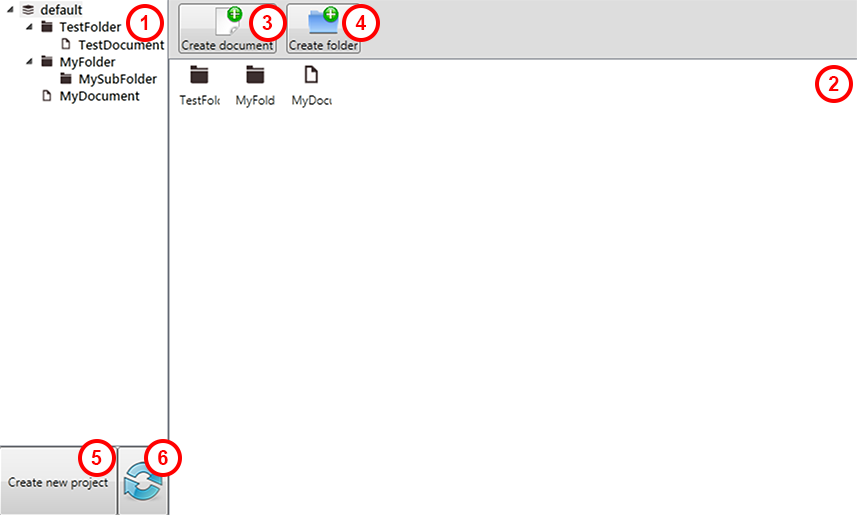
\includegraphics[width=1\textwidth]{User_manual/graphics/local.png}
	\caption{Screenshot of the local client}
	\label{fig:manual-local}
\end{figure}

You are not logged in, when you are using the local client, but it does require authentication whenever you wish to interact with online data.

\subsubsection{Projects}

	\paragraph{Create project}
	To create a new project, click the Create new project button (5 in figure~\ref{fig:manual-local}) and enter the desired name in the pop-up window. You can now find your new project in the explorer (1 in figure~\ref{fig:manual-local}).

	\paragraph{Share project}
	In order to share a project in the local client, you need to have an internet connection established and your data
    has to be synchronized at some point before, meaning you do not have to have an up-to-date project, folder or
    document, but the project has to exist online. When these requirements are fulfilled, you can right-click a project
    in the explorer (1 in figure~\ref{fig:manual-local}) and click Share project. This will open a pop-up window with
    a text field, which can handle both single email addresses or comma-separated lists of email addresses.

	\paragraph{Remove project}
	To remove a project, right-click the project in the explorer (1 in figure~\ref{fig:manual-local}) and click Remove project. Be aware that all subitems (folders and documents) will also be removed.

	\paragraph{Synchronize}
	In order to synchronize your data, you need to have an internet connection established. When that requirement is fulfilled, you can synchronize your data, by clicking the synchronize button (6 in figure~\ref{fig:manual-local}) and entering your account information in the pop-up window. If the user does not exist, a new one will be created with the desired account information. All data will then be synchronized, which can take several moments.

\subsubsection{Folders}

	\paragraph{Create folder}
	To create a new folder, click the Create folder button (4 in figure~\ref{fig:manual-local}) or right-click a project or folder in the explorer (1 in figure~\ref{fig:manual-local}) and click Create folder. Then enter the desired name in the pop-up window. You can now find your new folder in the explorer as a subitem under the project or folder under which it was created.

	\paragraph{Remove folder}
	To remove a folder, right-click the folder in the explorer (1 in figure~\ref{fig:manual-local}) and click Remove folder.  Be aware that all subitems (folders and documents) will also be removed.

\subsubsection{Documents}

	\paragraph{Create document}
	To create a new document, click the Create document button (3 in figure~\ref{fig:manual-local}) or right-click a project or folder in the explorer (1 in figure~\ref{fig:manual-local}) and click Create document. Then enter the desired name in the pop-up window. You can now find your new document in the explorer as a sub item under the project or folder under which it was created.
	
	\paragraph{Edit document}
	To edit a document, click on the document in the explorer (1 in figure~\ref{fig:manual-local}). This will open the document with a large editing area (1 in figure~\ref{fig:manual-local-document}). When editing the document, you can use the \emph{HyperText Markup Language}\cite{w3cHTML} (HTML) to format your content. To save the document, simply click the Save document button (2 in figure~\ref{fig:manual-local-document}).
	
	\begin{figure}[htb]
		\centering
		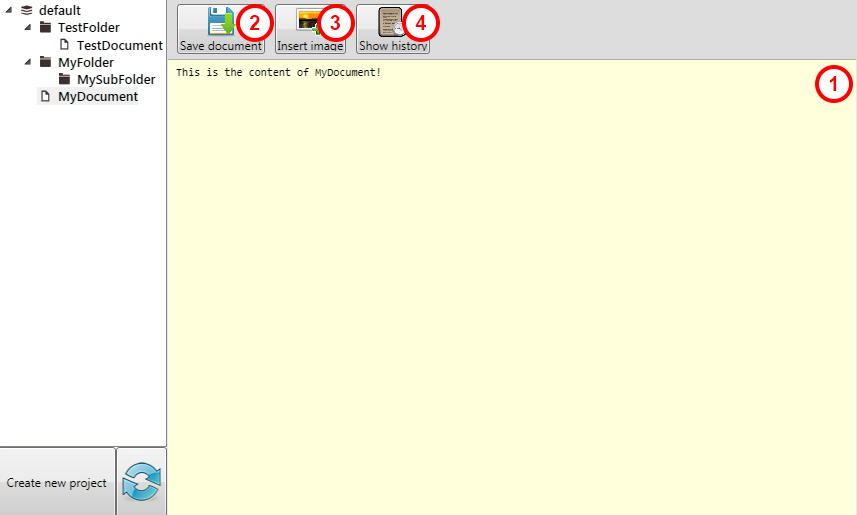
\includegraphics[width=1\textwidth]{User_manual/graphics/local-document.png}
		\caption{Screenshot of the document view in the local client}
		\label{fig:manual-local-document}
	\end{figure}
	
		\subparagraph{Insert image}
		To insert an image, click the Insert image button (3 in figure~\ref{fig:manual-local-document}) and enter the URL to the image in the pop-up window. This will insert an HTML image tag at the cursors position.
		
		\subparagraph{Show history}
		To view the revisions of a document, click the Show history button (4 in figure~\ref{fig:manual-local-document}). This will open a pop-up window with the most recent revision visible, while the rest of the history is available from the list in the left side of the window. You can copy the visible revision or part of it and paste it to your editor window.
	
	\paragraph{Remove document}
	To remove a document, right-click the folder in the explorer (1 in figure ~\ref{fig:manual-local}) and click Remove document. Be aware that all revisions will also be removed.
